\chapter{Estructura nuclear} \label{Ch:04}

\section{Introducción a la estructura nuclear}

Un núcleo atómico es un objeto constituido por muchos cuerpos (el Uranio tiene hasta 238 nucleones). Describir las propiedades nucleares a partir de la interacción básica entre esos cuerpos es una tarea formidable y fuera de nuestro alcanceen la actualidad por varias razones. En primer lugar la interacción entre dos nucleones no está del entendida desde el punto de vista teórico-conceptual\footnote{La Cromodinámica Cuántica (QCD) aunque ha superado pruebas experimentales, no permite hacer cálculos predictivos, y mucho menos deducir a partir de ella las características de interacción fuerte entre hadrones.}, y en segundo lugar, aunque dispusiéramos de una teoría completa que describiese la interacción en todos sus detalles no podríamos manejar operativamente el difícil problema de la interacción entre muchos cuerpos. Esto nos lleva de modo natural a intentar a describir la estructura nuclear y el espectro de excitaciones a partir de de modelos muy simplificados, esto es, modelos construidos a partir de algunas de las propiedades de los núcleos en lugar de las funciones de onda detalladas de cada nucleón. Se utiliza un planteamiento similar en la termodinámica, donde variables colectivas como la presión y la temperatura de un gas sustituyen a las variables cinemáticas de cada uno de sus átomos. A grandes rasgos, podemos clasificar los modelos de estructura nuclear en dos categorías:

\begin{itemize}
    \item \textbf{Modelos de fuerte correlación:} las propiedades nucleares sobre las que se construyen este tipo de modelos se explican como originadas a partir del comportamiento colectivo de los nucleones. Un ejemplo podrían ser los movimientos rotacionales y vibratorios nucleares, que dan lugar a espectros característicos de energía cuantizada. Es obvio que un movimiento rotatorio es un fenómeno creado por un comportamiento colectivo o correlacionado de los nucleones.
    \item \textbf{Modelo de casi nula corrección:} las características nucleares propias de estos modelos se suponen originadas por el comportamiento individual de cada nucleón.
\end{itemize}
Ninguno de los dos tipos de modelo en su versión extrema pueden explicar todas las propiedades nucleares. Los modelos más realistas tratan con una mezcla de propiedades colectivas e individuales de los nucleones. Un modelo basado exclusivamente en propiedades colectivas será insuficiente para explicar parte de las propiedades nucleares, y es necesario acudir a una cierta mezcla de propiedades colectivas e individuales para conseguir modelos nucleares con un rango de aplicación más interesante.

\section{El modelo de la gota líquida}

El modelo de la gota líquida lo hemos aplicado ya en un capítulo anterior para obtener la fórmula semiempírica de masas o fórmula de Weizsäcker, que nos permite calcular las masas y las energías de ligaduras de los núcleos. Una gota de líquido en ausencia de campos gravitatorios (o cualquier otro tipo de campo) adquiere una forma que minimiza la energía positiva de tensión superficial. Esta forma es la forma de la esfera. Una gota de líquido es esencialmente incompresible (su densidad es constante), y por lo tanto su radio será $R\sim n^{1/3}$, donde $n$ es el número de moléculas de la gota. Consideremos que la gota tiene una energía de ligadura\footnote{Las moléculas de la superficie estarán menos ligados que las interiores, pero este efecto se introduce como una corrección en términos de la tensión superficial.}  que podemos denotar por $a$ La energía de ligadura se debe a la interacción de la molécula con sus moléculas vecinas. Estas fuerzas de interacción se anulan a distancias grandes y se hacen repulsivas a distancias cortas comparadas con la distancia intermolecular típica\footnote{La interacción fuerte entre nucleones tiene características similares en cierto sentido, como veremos más adelante.}. Si tomamos como cero la energía la situación en la cual todas las moléculas de la gota están infinitamente separadas, podemos expresar la energía de ligadura de la gota (tomada positiva) de la siguiente manera:

\begin{equation}
    B=an - 4 \pi R^2 T = an-\beta n^{2/3} \quad (R^2 \sim n^{2/3})
\end{equation}
donde $T$ es la energía de tensión superficial del líquido. Si la gota tuviese una carga eléctrica $Q$ uniformemente distribuida en todo su volumen debemos añadir un término correspondiente a la energía potencial coulombiana:

\begin{equation}
    B = an - \beta n^{2/3} - \frac{\gamma Q^2}{n^{1/3}}
\end{equation}
donde $\gamma$ contiene todas las contantes de la energía coulombiana excepto la dependencia con $Q$ y $n$. 

Para obtener la fórmula de Weizsäcker, o fórmula semiempírica de masas, aplicamos estas ideas y algunas otras hipótesis de trabajo que recapitulamos aquí:

\begin{itemize}
    \item Suponemos un núcleo esférico.
    \item Los nucleones dentro del núcleo se comportan de modo análogo a moléculas en una gota líquida, es decir, fuerzas atractivas de corto alcance los mantienen unidos y fuerzas repulsivas, de todavía más corto alcance, los mantienen alejados unos de otros.
    \item La densidad nuclear es constante. 
    \item Existe una tendencia a mantener un número de protones muy parecidos al número de neutrones en un núcleo.
    \item Existe una \textit{fuerza de apareamiento} que favorece la existencia de núcleos con $Z$ par y $N$ par.
\end{itemize}

\section{El modelo de Gas de Fermi}

Alrededor de 1948, se comenzó a considera en serio la evidencia acumulada sobre la existencia de ciertos \textbf{números mágicos} para los valores de $Z$ Y $N$. La energía de separación de dos protones para secuencias de isótonos ($N$ constante) graficada como desvaiciones de la predicción de la fórmula semiempírica de masas, mostraba unos picos acusados par $Z=8,20,28,50,83$; mientras que la energía de separación de dos neutrones para secuencias de isótopos, también graficada como desviaciones de la predicción de la fórmula semiempírica de masas muestra picos para $N=8,20,28,50,82,126$. La similitud de estas gráficas con la de algunas propiedades atómicas, como la energía de ionización es sorprendente. Recordemos que estas propiedades atómicas tienen su origen en la formación de \textit{capas cerradas} de electrones moviéndose \textit{independientemente} en un potencial efectivo atómico. Sin resistencia a pesar que los nucleones se puedierar mover independientemente en el núcleo sin interaccionar (o apenas interaccionando) los unos con los otros, sobre todo debido al éxito del modelo nuclear de la gota líquida en la explicación aproximada de las masas de los núcleos.

Los datos experimentales indican que los nucleones parecen comportarse de dos maneras contradictorias: por un lado, como un grupo de partículas fuertemente interaccionantes en un especie de estado condensado con características similares a las de un líquido, y por otro como un sistema de partículas que apenas interaccionan entre sí, con características propias de un gas. A la hora de comprender estas características aparentemente contradictorias resultas útil introducir la abstracción de \textbf{materia nuclear} sin repulsión coulombiana, y tan grande que pudiésemos despreciar los efectos de superficie. Weisskopf fue el primero en tratar de explicar las propiedades de la materia nuclear por medio del modelo del \textbf{gas de Fermi}, en completo analogía con el modelo que se usa para explicar las propiedades de conducción eléctrica de los metales considerando un \textit{gas de electrones libres}.

Se supone que cada nucleón se mueve libremente en un pozo de potencial neto atractivo creado por todos los demás nucleones. Este potencial neto tiene una profundidad constante en el núcleo puesto que la distribución de nucleones es constante en esta región, y se aproxima a cero rápidamente en una distancia que coincide con el rango del alcance de la fuerza nuclear fuerte. Cuando el núcleo se encuentra en su estado fundamental todos los nucleones ocupan los niveles más bajos de energía del pozo de potencial y el llenado de niveles se realiza de acuerdo con el principio de exclusión de Pauli. Esto significa que no es posible que exista transferencia de energía (interacción) entre dos nucleones, porque ello supondría desplazarlos de sus niveles energéticos y estamos asumiendo que todos los niveles están ya ocupados\footnote{Un intercambio de niveles entre dos nucleones no representa ninguna interacción, porque los nucleones son indistinguibles.}. Únicamente sería posible que uno de los nucleones saltase a uno de los niveles de valencia desocupados, pero eso requiere más energía de la habitualmente disponible en el movimiento de los nucleones dentro de un núcleo en su estado fundamental.


Podemos entonces suponer de forma aproximada que los nucleones se encuentran en un pozo esférico de potencial cuyo perfil puede verse esqumáticamente en la figura \ref{Fig:04-01}. Para un núcleo de $A \sim 100$ el radio del pozo de potencial sería $R_c \sim$5.6 fm, lo cual es suficientemente para evitar que los efectos de superficiie sean los dominantes. En este esquema simplificado, el pozo de potencial para los protones no es el mismo que para los neutrones. El de los protones es un poco menos profundo debido a la repulsión coulombiana que ellos sienten y los neutrones no. Además, para los protones tenemos una barrera coulombiana que alza el extremo superior del pozo unas decenas de MeV (nótese la línea roja, que es la región del potencial de protones).

\begin{figure}[h!] \centering
	\begin{pspicture}(-1,-5)(6,3)
		\psline[arrowscale=2,linewidth=1pt]{->}(0,-4)(0,3)
		\psline[linewidth=1pt](0,-4)(2,-4)
		\psline[linewidth=1pt](2,-4)(2,0)
		\psline[arrowscale=2,linewidth=1pt]{->}(2,0)(6,0)
		\psline[linewidth=0.9pt](0,-0.4)(2,-0.4)
		
		\psline[linewidth=0.9pt,linearc=2,linecolor=red,linestyle=dashed](0,-3)(1,-3.5)(2,-3.5)
		\psline[linewidth=0.9pt,linearc=2,linecolor=red,linestyle=dashed](2,1)(3.5,0.1)(5,0.1)
		\psline[linewidth=0.9pt,linearc=2,linecolor=red,linestyle=dashed](2,0)(2,1)
		\psline[linewidth=0.9pt,linearc=2,linecolor=red,linestyle=dashed](0,-0.6)(2,-0.6)
		
		\rput(2.5,1.5){\textcolor{red}{{\small Pozo de protones}}}
		\rput(1.0,-4.5){{\small Pozo de neutrones}}
		
		\rput(-0.4,2.0){V(r)}
		\rput(5.0,-0.5){r}
		
		\psline[linewidth=0.75pt,arrowscale=1]{<->}(0,-1.2)(2,-1.2)
		\rput(1.0,-1){$R_c$}
		
		\psline[linewidth=0.75pt,arrowscale=1]{<->}(2.2,-4)(2.2,-0.4)
		\rput(4.0,-2){{\footnotesize  $E_f \sim 33 \ \unit{\MeV}$ (neutrones)}}
		
		\psline[linewidth=0.55pt,arrowscale=1]{<->}(2.5,-0.4)(2.5,-0.0)
		\rput(3.2,-0.2){{\footnotesize  $\sim 8 \ \unit{\MeV}$}}
		
		
	\end{pspicture}
	\caption{Aproximación del potencial por un pozo.}
	\label{Fig:04-01}
\end{figure}

Los nucleones llenarían sus respectivos niveles energéticos en estos pozos de potencial de acuerdo con el principio de exclusión de Pauli hasta una energía cinética máxima conocida como \textbf{energía de Fermi}, $E_F$. Esta energía se puede estimar suponiendo un núcleo de volumen $4\pi R^3/3$ y número de nucleones constituyentes conocido. A la energía de Fermi le corresponde un momento de Fermi dado por $E_F=p_F^2 / 2m$, y un volumen en el espacio de momentos $V_p=4\pi p_F^2/3$, de tal manera que el volumen disponible en el espacio de fases sería:

\begin{eqnarray}
	V_{\text{ef}} = \parentesis{\frac{4}{3}\pi}^2 (r_0 p_F)^3 A 
\end{eqnarray}
donde $r_0 \sim 1.2 $ fermis y $A$ es el número másico. Ahora bien, de acuerdo con el principio de Heisenberg el mínimo volumen en el espacio de fases que se puede asociar a un estado físico de cualquier sistema es $V_{\text{ef-min}}\sim h^3$ (siendo $h$ la constante de Planck), por lo tanto el número de nucleones que se puede acomodar en el volumen del espacio de fases hasta el nivel de Fermi, teniendo en cuenta el factor 2 debido a fermiones de espín 1/2 será:

\begin{eqnarray}
	n_F = \frac{2}{\hbar^3}V_{\text{ef}} = \frac{4}{9\pi} \parentesis{\frac{r_0 p_F}{\hbar}}^3 A
\end{eqnarray}
Si ahora tomamos en consideración la situación habitual en que $Z=N=A/2$ y por lo tanto $n_F=A/2$ entonces conseguimos la siguiente estimación para el momento y la energía de Fermi:

\begin{eqnarray}
	p_F = \frac{\hbar}{r_0} \parentesis{\frac{9\pi}{8}}^{1/3} \quad E_F = \frac{p_F^2}{2m} = \frac{1}{2m} \parentesis{\frac{\hbar}{r_0}}^2 \parentesis{\frac{9\pi}{8}}^{2/3} \sim 33\ \unit{\MeV}
\end{eqnarray}
Concluimos por tanto que para los neutrones podemos tomar aproximadamente $E_F\sim 33 \ \unit{\MeV}$ e independiente de $A$. Por otro lado, el nivel de energía de Fermi debe coincidir con el nivel que ocupe el nucleón menos ligado, que está a una distancia del nivel de energía cero (situación en la que el nucleón no está ligado al núcleo) igual a la energía de separación. La profundidad del pozo de neutrones será igual entonces a la suma de la energía de Fermi ($\sim 33 \ \unit{\MeV}$) más la energía de separación ($\sim 8 \ \unit{\MeV}$), lo cual nos da unos 40 MeV. Es interesante reflexionar sobre el hecho de que únicamente a partir del tamaño nuclear y del principio de incertidumbre podamos estimar la profundidad del pozo de potencial nuclear. 


A pesar de que las profundidades en los pozos de protones y neutrones son distintas, lo que provoca por ejemplo que los núcleos con $N>Z$ sean mas estables que con $Z>N$, las energías de Fermi deben estar aproximadamente en la misma posición por debajo del valor cero en el pozo de potencial, de lo contrario no habría estabilidad, y la energía de separación del último nucleón sería dependiente de la carga, lo cual estaría en contradicción con las observaciones experimentales.





\section{El modelo de capas}

A semejanza del modelo atómico de capas que tanto éxito a tenido en la física atómica, resulta tentador preguntarse si un modelo similar no tendría éxito también en la física nuclear. Es necesario, sin embargo, tener en cuenta las profundas diferencias entre la física atómica y la nuclear. 

Los electrones se mueven en un potencial externo aproximadamente central: el potencial que crea el núcleo junto con las correcciones oportunas debidas al resto de electrones. De este modo manera surgen natural las capas electrónicas, que se van llenando en orden de energía creciente cumpliendo el principio de exclusión de Pauli. Las capas electrónicas llenas forman una especie de zona interior neutra y los electrones de la capa semillena constituyen los electrones de valencia, que determinan la mayoría de las propiedades químicas del átomo correspondiente. Cuando vamos llenando una capa electrónica las propiedades atómicas como la energía de ionización varían suavemente, pero sufren una súbita discontinuidad cuando la capa queda llena y hemos de pasar a la siguiente. 

En un núcleo no tenemos un agente externo que cree el potencial en el que se mueven los nucleones, son ellos mismos los que configuran el potencial efectivo nuclear. Otra compilación o diferencia adicional es que, en principio, parecería que los nucleones debieran tener una probabilidad no despreciable de colisionar los unos con los otros, mientras que eso no sucede con los electrones atómicos. No resulta evidente que podamos considerar a cada nucleón moviéndose independientemente de los demás en un potencial nuclear efectivo, pero ya hemos visto que el principio de exclusión de Pauli garantiza que, esencialmente, los nucleones se mueven libremente dentro del núcleo. 

La hipótesis principal del modelo de capas es suponer que los nucleones se mueven en el núcleo casi independientemente los unos de los otros a pesar de la interacción fuerte. Este movimiento libre significa, en última instancia, que el recorrido libre medio de un nucleón en materia nuclear es grande comparado con las dimensiones del núcleo. En el modelo de capas la interacción nucleón con sus compañeros se reduce a la interacción con un \textbf{campo autoconsciente} (\textit{self-consistent field}) creado por ellos. Generalmente se supone que este campo autoconsciente es estático y esféricamente simétrico.

Debido al corto alcance de las fuerzas nucleares, el potencial del campo autoconsciente tiene dependencia radial muy similiar a la densidad nuclear, es decir, es casi constante dentro del núcleo y se anula fuera. Por lo tanto, en primera aproximación podríamos considerar que el potencial nuclear constante en el interior del núcleo, tal como se hace en el modelo de gas de Fermi ideal\footnote{El modelo de capas incorpora la hipótesis del modelo de gas de Fermi.}, con lo cual las funciones de onda de los nucleones serían ondas planas. No obstante, la introducción den el modelo de capas de un campo autoconsistente que depende de la distancia al centro del núcleo es una mejora sustancial respecto del modelo de gas de Fermi, y modifica las funciones de onda de los nucleones, dejando de ser ondas planas. 

Existen varias versiones del modelo de capas. La más simple, conocida como \textbf{versión extrema del modelo de capas} (\textit{one-particle shell mode}), se usa para explicar las propiedades de los núcleos con $A$ impar. En esta versión se supone que todos los nucleones están apareados (incluyendo los de una hipotética capa semillena) formando una coraza interde de espín cero, y que las propiedades del núcleo se deben únicamente al estado del nucleón desapareado. Una mejora de este modelo consiste en considerar todos los nucleones de la última capa semillena, no sólo el desapareado. El siguiente paso en la elaboración de un modelo más detallado sería, obviamente, considerar todos los nucleones, tanto en las capas llenas como las semillenas.

\subsection{Evidencia experimental de capas en los núcleos}

Hemos visto que para ciertos valores mágicos de $N$ y $Z$ los núcleos muestran una estabilidad inusual, que se manifiesta, por ejemplo, en una energía de separación de dos nucleones (protones o neutrones) grande. Además cuando $Z$, o $N$, o ambos, coinciden con un número mágico, la energía de ligadura nuclear es mayor que la esperada y algunas otras propiedades nucleares, como el radio, se comportan como si se hubiera completado una capa de estados análoga a las capas electrónicas atómicas. El modelo de capas nuclear considera niveles energéticas de los nucleones en un potencial adecuado. Una capa consiste en un grupo de niveles energéticos cercanos. A continuación se ofrece alguna lista de algunas evidencias experimentales en favor de la existencia de números mágicos:

\begin{itemize}
	\item Existen grandes desviaciones en la energía de ligadura nuclear cerca de los números mágicos. 
	\item La energía de separación protónica (neutrónica) tiene picos cuando $Z$ ($N$) es mágico.
	\item La energía cinética de las partículas $\alpha$ es particularmente alta cuando el núcleo hijo tiene un número mágico de neutrones.
	\item Los elementos con $Z(N)$ mágico tienen más isótopos (isótonos) que sus vecinos.
	\item El primer estado excitado $2^+$ de un núcleo par-par tiene una energía excepcionalmente alta si $z$ y $N$ son mágicos.
	\item El radio nuclear decrece en los núcleos con $N$ mágico.
	\item La sección eficaz de captura de neutrones decrece en unos dos órdenes de magnitud para los núcleos con $N$ mágico.
\end{itemize}


Como ya hemos mencionado, la hipótesis fundamental del modelo de capas es ésta: cada nucleón se mueve independientemente de los demás en un potencial creado por todos los otros nucleones. Una vez definido el potencial, tratando cada nucleón de esta manera podemos ir llenando los niveles energéticos de acuerdo con el principio de Pauli. Este mismo principio es el que garantiza en cierto modo la existencia de algo parecido a \textit{órbitas} individuales\footnote{Órbitas en el sentido clásico no existen, aquí nos referimos al hecho de considerar el movimiento individual de cada partícula} de cada nucleón. Supongamos la colisión se encuentran cerca del fondo de potencial. Si las energéticas superiroes están llenas ya de nucleones, el único modo de que haya trasferencia de energía en la colisión es que uno de los dos nucleones sea promovido a la capa de valencia, pero esto requiere más energía que la disponible en una colisión de este tipo, con lo cual el resultado final es que, al menos como primera aproximación, los nucleones no colisionan los unos con los otros y se mueven individualmente por el potencial efectivo nuclear\footnote{El recorrido libre medio de un nucleón de 10 MeV en una reacción nuclear es alrededor de 2 fm en materia nuclear, lo cual es muy poco y podría parecer que entra en contradicción con nuestra hipótesis. No obstante, nuestra discusión anterior se aplica sólo a nucleones ligados, donde tiene aplicabilidad el principio de Pauli. Esto no ocurre para nucleones no ligados como un nucleón proyectil que intervenga en una reacción nuclear}.

\subsection{Modelo de capas con potencial armónico}

Dos candidatos simples para el potencial nuclear podrían ser el pozo de potencial esférico de paredes infinitas o el oscilador armónico en tres dimensiones. En ambos casos tenemos solución anlítica para la ecuación de Schrödinger

\begin{eqnarray}
	\ccorchetes{-\frac{\hbar^2}{2m} \nabla^2 + V(r)} \Psi (\rn) = E\Psi (\rn)
\end{eqnarray}

Para un potencial central las soluciones de esta ecuación podemos escribirlas como

\begin{eqnarray}
	\Psi_{n\ell m} (\rn) = \frac{u_{n \ell} (r)}{r} Y_{\ell}^m (\theta,\varphi)
\end{eqnarray}
donde los $Y_{\ell}^m (\theta,\varphi)$ son los armónicos esféricos, y $u_{n\ell}$ las ondas radial. En el caso especial del potencial tridimensional isótropo tenemos:

\begin{eqnarray}
	V(r) = \frac{1}{2} m \omega^2 r^2
\end{eqnarray}
y los autovalores vienen dados por

\begin{eqnarray}
	E_N = \parentesis{N+ \frac{3}{2}}\hbar \omega = \parentesis{2n + \ell - \frac{1}{2}} \hbar \omega \quad N=0,1,2...
\end{eqnarray}
\begin{eqnarray}
	N=2(n-1)+\ell \quad n=1,2,3\ldots \quad \ell = 0,1,2,\ldots \quad (-1)^{\ell} = (-1)^N \ \ell \leq N
\end{eqnarray}
La energía depende únicamente de $N$, denominado número cuántico principal, que es el que se obtiene de manera más directa resolviendo la ecuación de Schrödinger para el oscilador armónico tridimensional en coordenadas cartesianas. De acuerdo con estas ecuaciones, el espectro energético de una partícula en un potenciala armónico consiste en una secuencia de niveles equidistantes separados por $\hbar \omega$. A cada nivel $E_N$ le corresponden varios estados con diferentes valores de $\ell$. Los enteros $\ell$ y $N$ tienen siempre la misma paridad y $\ell \leq N$. Se puede comprobar fácilmente que la degeneración es:

\begin{eqnarray}
	g_N = \frac{1}{2}(N+1)(N+2)
\end{eqnarray}
A esto habría que añadirle un factor 2 correspondiente a la degeneración de espín, ya que los nucleones son fermiones de espín 1/2. Los diferentes estados pueden identificarse con el par de números ($n \ell$), o bien mediante la notación espectroscópica ($s,p,d,f,g,h\ldots$) de tal manera que hablemos de $1s,2d,2g\ldots$. \\


Podemos intentar refinar un poco el potencial propuesto, porque es evidnete que el pozo nuclear no puede ser de paredes infinitas, y el potencial armónico no parece decrecer con la suficiente rapidez. Un potencial más realista sería el \textbf{potencial Wood-Saxon}:

\begin{eqnarray}
	V(r) = - \frac{V_0}{1+\exp [(r-R)/a]}
\end{eqnarray}
cuyo perfil se muestra en la figura \ref{Fig:04-02}. Los parámetros $R$ y $a$ representan el radio medio y el \textit{skin thikness} respectivamente. Sus valores se escogen de acuerdo con los datos experimentales que indican $R=\num{1.25} A^{1/3} \ \unit{\fm}$ y  $a=0.524 \ \unit{\fm}$. La profundidad del pozo, $V_0$, se ajusta para que proporcione  energías de separación adecuadas, y es del orden de $V_0\sim 40 \ \unit{MeV}$. El efecto de este potencial, comparado con el del oscilador armónico, consiste en destruir la degeneración $\ell$ de las capas. El desplazamiento energético entre subniveles aumenta a medida que crece la energía de excitación, y eventualmente se hace tan grande como el propio espaciamiento entre las capas. En cualquier caso, seguimos sin obtener más números mágicos que los tres primeros. 


\begin{figure}[h!] \centering
	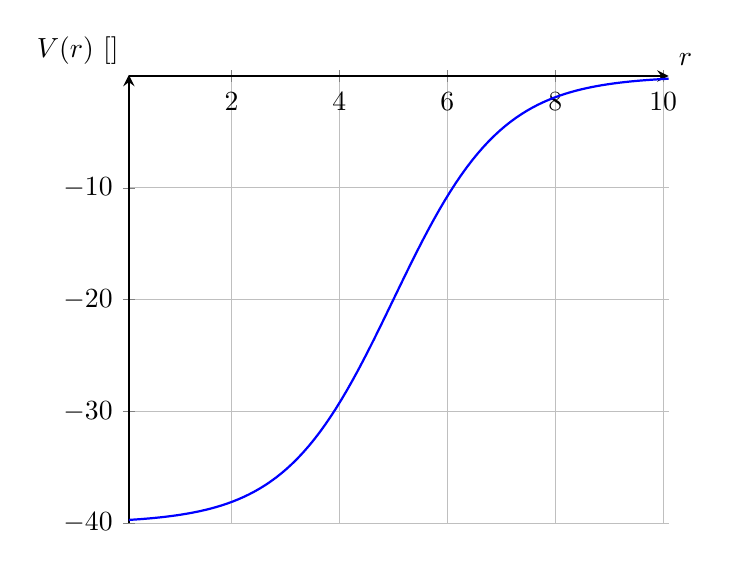
\begin{tikzpicture}
		\begin{axis}[
			domain=0.1:10.1,    % Rango del dominio para r > 0
			samples=100,    % Número de muestras para hacer la curva suave
			axis lines=middle,    % Líneas del eje
			xlabel={$r$},    % Etiqueta del eje x
			ylabel={$V(r) \ [\unit{\MeV}]$},    % Etiqueta del eje y
			ymin=-40.0, ymax=0.1,  % Límites del eje y
			xtick={2,4,6,8,10},       % Marcar el punto r=1
			ytick={-10,-20,-30,-40},      % Marcar el valor V(r) en r=1
			xlabel style={above right},
			ylabel style={above left},
			grid=both,
			thick
			]
			\addplot[
			blue,
			thick
			] {-(40/(1+exp(x-5)))};  % Punto de referencia
		\end{axis}
		
%		\draw[thick] (1.75,6.1) -- (5.2,6.1);
	%	\node (A) at (3.8,6.4) {$S_{\text{thick}}$};
	\end{tikzpicture}
	\caption{Potencial Wood-Saxon, variables de distancia en coordenadas reducidas ($R = 5, \ a = 1$).}	
	\label{Fig:04-02}
\end{figure}

\subsection{Interacción espín-órbita}

En los años 40 del siglo XX se realizaron muchos esfuerzos para constuir un modelo de estructura nuclear que explicase de los números mágicos. En 1949 Mayer, Haxel, Suess y Jensen probaron que la inclusión de un potencial de interacción espín-órbita producía el desdoblamiento correcto de los subiveles en las capas. En física atómica la intearcción espín órbita tiene su origen en la interacción del momento dipolar mangético creado por el espín del electrón con el campo mangnético que el electrón ve en su propio sistema de referencia\footnote{En el sistema de referencia en que el electrón está en reposo y el núcleo atómico está en movimiento y genera un cmapo magnético que interacciona con el momento dipolar magnético del electrón.}; los efectos aquí son típicamente del orden de una parte entre $10^5$, demasiado pequeños como para generar un desdoblamiento energético que modifique los \textit{números mágicos atómicos}. En el caso del nucleo veremos que la interacción espín-órbita si introduce cambios significativos en lo que conciernte a la secuencia de números mágicos. 

Introducimos entonces una interacción espín-órbita en el potencial nuclear de la siguiente manera:

\begin{eqnarray}
    V(r) \longrightarrow V(r) + V_{so} (r) \parentesis{\lnn \cdot \sn}
\end{eqnarray}
El factor $V_{so} (r)$ no es el más importante aquí, el que causa el desdoblamiento es el término $\lnn\cdot\sn$. Los estados de cada partícula se tienen que etiquetar ahora como el número cuántico correspondiente al momento angular total $\jn =\lnn+\sn$. Como los nucleones tienen $s=1/2$, los posibles valores de $j$ para un nucleón son $j=\ell\pm 1/2$, excepto para $\ell=0$ que solo es posible $j=1/2$. Podemos calcular el valor esperado de la expresión $\lnn \cdot \sn$ como:

\begin{eqnarray}
    \jn^2 = \lnn^2 + 2 \lnn\cdot\sn + \sn^2 \Rightarrow \lnn \cdot \sn = \frac{1}{2} \parentesis{\jn^2 -\lnn^2 -\sn^2}     
\end{eqnarray}
\begin{eqnarray}
    \langle \lnnn \cdot \sn \rangle = \frac{\hbar^2}{2} \ccorchetes{j(j+1)-\ell(\ell+1) - s(s-1)}
\end{eqnarray}
Supongamos ahora el nivel $1f$ ($\ell = 3$), que tiene una degeneración total $2(2\ell+1)=14$ (a cada uno le corresponde una degeneración diferente). Los posibles valores de $j$ son $j=\ell \pm 1/2=5/2$ o $7/2$, lo que nos da los dos estados $1f_{5/2}$ y $1f_{7/2}$, que constituyen un doblete espín-órbita y están degenerados y están separados por una energía proporcional al valor de $\langle \lnn \cdot \sn \rangle$. Para cada uno de estos dos orbitales tenemos una degeneración $(2j+1)$ proveniente de los distintos valores que $m_j$ puede tomar, lo cual proporciona una capacidad de 6 estaos nucleares para el $1f_{5/2}$ y 8 para el $1f_{7/2}$. Un total de 14, que coincide con el número inicial (el número total de estados no puede cambiar). Para cada par de estados de un doblete espín órbita con $\ell \neq 0$ tenemos una energía de separación proporcional a

\begin{eqnarray}
	\langle \lnn \cdot \sn \rangle_{j=\ell+1/2} - \langle \lnn \cdot \sn \rangle_{j=\ell-1/2} = \frac{\hbar^2}{2} (2\ell +1)
\end{eqnarray}
La fórmula anterior implica que la separación energética aumenta a medida que crece $\ell$ . Si tomamos $V_{so} (r)$ negativo, el miembro del par con mayor $j$ se desplaza hacia abajo entre los niveles de la segunda y tercera capas. Los 8 nucleones que puede contener el orbital $1f_{7/2}$ se podrían añadir a los 20 de las tres primeras capas generando un número mágico 28. De manera análoga es posible generar todos los números mágicos observados. \\

Existen varias secuencias de llenado de nucleones en la literatura, dependiendo de los parámetros exactos que se usen en la parametrización del campo nuclear autoconsciente. La que aparece en el libro de K. Krane (las barras verticales indican las separaciones entre capas que dan lugar a los números mágicos 2,8,28,50,82):

\begin{eqnarray}
	\begin{array}{l}(1s_{1/2})^2 \ || \ (1p_{3/2})^4 (1p_{1/2})^2 \ || \ (1d_{5/2})^6 (2s_{1/2})^2 (1d_{3/2})^4 \ || \ (1f_{7/2})^8 \ || \ (2p_{3/2})^4 \\ (1f_{5/2})^6 (2p_{1/2})^2 (1g_{9/2})^{10} \ || \ (1g_{7/2})^8 (2d_{5/2})^6 (1h_{11/2})^{12}  (2d_{3/2})^4 (1h_{9/2})^{10} \\ (1i_{13/2})^{14} \ || \ (2g_{9/2})^{10} (3d_{5/2})^6 (1i_{11/2})^{12}  (2g_{7/2})^8 (4s_{1/2})^2 (2d_{3/2})^4  (1j_{15/2})^{16} \ ||		\ldots
	\end{array}
\end{eqnarray}
De tal modo que $(1p_{3/2})^4$ indica el primer llenado del orbital $p$ ($\ell=1$), con espín total $3/2$ ($j=\ell + s$) con degeneración total 4 (la degeneración es $2j+1$). 

\subsection{Modelos dipolares magnéticos}

En la versión extrema del modeleo de capas (\textit{one-particle shell model}), el momento dipolar magnético de un núcleo con $A$ impar está determinado por el momento dipolar magnético del último nucleón desapareado. Veamos cuál es el acuerdo que existe entre los datos experiementales y este modelo. Recordemos que el operador de momento magnético dipolar para un núcleo de $A$ nucleones se escribe como

\begin{eqnarray}
	\mun = \frac{\mu_N}{\hbar} \sum_{i=1}^A \ccorchetes{g_i^{(\ell)} \lnn_i + g_i^{(s)}\sn_i} \tquad \mu_N = \frac{e\hbar}{2m_p}
\end{eqnarray}
donde $\mu:N$ es el magnetón nuclear y los valores para los fotones o razones giromagnéticos correspondientes al momento angular orbital y al de espín, para el fotón neutrón y electrón son:

\begin{eqnarray}
	g_p^{(\ell)} = 1 & & g_p^{(s)} = \num{5.585694674} \\
	g_n^{(\ell)} = 0 & & g_p^{(s)} = \num{-3.8260854} \\
	g_e^{(\ell)} = -1 & & g_p^{(s)} = \num{2.002319304374} \\
\end{eqnarray}
El momento dipolar magnético del núcleo se define como el valor esperado de la tercera componente del operador $\mun$ en un estado nuclear en el que la proyección del momento angular sobre el eje $z$ es máxima, es decir, cuando $j_z=j\hbar$. En la versión extrema del modelo de capas se pretende explicar el momento magnético nuclear como originado por el único nucleón desapareado (sólo para núcleos de $A$ impar). Considerando entonces la contribución de un único nucleón, la tercera componente del operador anterior es:

\begin{eqnarray}
	\mu_z = \frac{\mu_N}{\hbar} \parentesis{g^{(\ell)} \ell_z + g^{(s)} s_z}
\end{eqnarray}
La presencia de interacción espín-órbita implica que el potencial es no central, y por lo tanto los autoestados del hamiltoniano no lo serán también del operador momento angular orbital, sino del momento angular total. Esto quiere deecir que $\ell_z$ y $s_z$ ya no serán \textit{buenos} números cuánticos, hemos de usar $\jn=\lnn+\sn$ y $j_z$. Podemos reescribir la expresión anterior usado la tercera componente de $\kn$ de la siguiente manera (recordando que $\j_z=\ell_z + s_z$):

\begin{eqnarray}
	\mu_z = \frac{\mu_N}{\hbar} \ccorchetes{g^{(\ell)}j_z + (g^{(s)}-g^{(\ell)})  s_z}
\end{eqnarray}
Tomamos el valor esperado de la experiencia anterior cuando $j_z=j\hbar$, y para aligerar notación preescidimos del subíndice $z$ y $\mu$ sobreentendiendo que se trata de la tercera componente:
\begin{eqnarray}
	\langle \mu_z \rangle = \frac{\mu_N}{\hbar} \ccorchetes{g^{(\ell)} \langle j_z \rangle + (g^{(s)}-g^{(\ell)}) \langle s_z \rangle}
\end{eqnarray}
Obtenemos así de nuevo estas dos expresiones para el momento dipolar magnético:

\begin{eqnarray}
	\mu_{j=\ell+\frac{1}{2}} & = & \frac{\mu_N}{2} \ccorchetes{(2j+1)g^{(\ell)} + g^{(s)}} \\
	\mu_{j=\ell-\frac{1}{2}} & = & \frac{\mu_N}{2} \frac{j}{j+1} \ccorchetes{(2j+1)g^{(l)} - g^{(s)} }
\end{eqnarray}

